\chapter{Python Tutorial}
\label{PythonTutorial}
\graphicspath{{figures/Python/}}
 This tutorial is available as a Jupyter notebook (extension .ipynb). Note that this tutorial is made for \textbf{Python 3.x} and is not compatible with older Python versions. Make sure you are working with an appropriate version!

\section{What are Python and Jupyter Notebooks?}
\textbf{Python} is a programming language used to write computer programs. These programs consist of lines of code that can be interpreted and executed by a computer one by one. Like all (programming) languages, Python has its own vocabulary and grammar. This is called the \textbf{syntax}, i.e. \ the rules that the code must follow in order for computers to be able to read it. \\

Here we use Python in a \textbf{Jupyter Notebook}, available through a web browser (Jupyter.org). Jupyter Notebooks are structured in so-called cells. We distinguish two types of cells: 

\begin{enumerate}
	\item \textbf{Markdown cells} contain text with titles, explanations, assignments,\ldots . This text is entered as code, which is converted to formatted text when executed.
	
	\item \textbf{Input cells} contain Python code that can be executed. In front of such cells you see \lstinline|In [x]:|, where x keeps track of the number of cells executed. When the cell is executed, the output(s) appear below the input cell. These are then preceded by \lstinline|Out [x]:|.
\end{enumerate}

Two modes are possible for a cell:

\begin{enumerate}
	\item \textbf{Command Mode} (left bar is blue): in this mode, operations can be done on the entire cell (e.g. changing cell type, cutting and pasting cells, inserting cells,...).
	
	\item \textbf{Edit Mode} (left bar is green): in this mode, the text/code in the cell can be edited.
\end{enumerate}

Press \keystroke{Enter} to switch to edit mode and press \keystroke{Esc} to switch back to command mode. Use \keystroke{Ctrl} + \keystroke{Enter} to enter a cell, and \keystroke{Shift} + \keystroke{Enter} to select the cell below after entering. An overview of commands for both modes is listed under Help > Keyboard Shortcuts.

\paragraph{Question 1} 
What should you enter to create a new Input cell under an existing cell? And in what mode should you enter this? Enter your answer below and convert this cell back to formatted text.
\begin{JupyterMarkdown}
	Answer: \ldots
\end{JupyterMarkdown}

\paragraph{Question 2}
Create an Input cell below with the command
\begin{center}
	\lstinline|print("Hello, world!")|
\end{center}
and enter this cell.

\section{Python for dummies}
\subsection{Objects}
Python is a so-called object-oriented programming language, which means that we perform operations on objects. The operations covered here are mainly mathematical ones. Objects are data stored in computer memory. Each object has a particular class, which determines which operations can be performed on it. The object class can be checked with the command \lstinline|type|.

\begin{lstlisting}[]
>>> type(1)
int
>>> type(1.5)
float
\end{lstlisting}

The examples above are both numbers, yet belong to different object classes! \lstinline|1| is an integer, whereas \lstinline|1.5| is a is a so-called floating point number. Note that Python distinguishes these two classes from each other by the presence or absence of a decimal sign.

\begin{lstlisting}[]
>>> type(1.)
float
\end{lstlisting}

Besides number objects, other types exist as well. A first example is a so-called \lstinline|list|. This datatype stores a set of objects together in an ordered sequence, indicated by square brackets \lstinline|[]|. A second example is the data type \lstinline|string|, which is used to store text. Strings are indicated by single (\lstinline|'|) or double (\lstinline|"|) quotation marks. Text not between quotation marks is interpreted as a command.

\begin{lstlisting}[]
>>> [1,1.5,2]
[1,1.5,2]

>>> type([1,1.5,2])
list

>>> type("This is a string.")
str

>>> type('This is a string as well.')
str

>>> This is not a string and will thus result in an error.
        File "<ipython-input-5-ec99100478b7>", line 1
          This is not a string and will thus result in an error.
                           ^
     SyntaxError: invalid syntax
\end{lstlisting}

\subsection{Variables}

Often we want to store a certain object (temporarily), in order to use it further. To do this, we use variables. A variable is a name we assign to a particular object in computer memory. This is done as follows: 
\lstinline|variable_name = object|.

\begin{lstlisting}[]
>>> a=1
    a
1
\end{lstlisting}

In the cell above, a value of 1 is assigned to the variable \lstinline|a| on the first line. This operation gives no output. When we call \lstinline|a| again, we get a value of 1 as output. Keep in mind the order! When assigning, the name of the variable must always be to the left and that of the object to the right of "=". Otherwise we get an error message.
\begin{lstlisting}[]
>>> 1 = a
        File "<ipython-input-14-7596acd8e627>", line 1
         1 = a
              ^
      SyntaxError: can't assign to literal
\end{lstlisting}

Variables can also be overwritten, which means that we assign a new object to the name of the variable.

\begin{lstlisting}[]
>>> a = 2
    a
2
\end{lstlisting}

Moreover, to determine the new object in the variable, reference can be made to the current object linked to the variable.

\begin{lstlisting}[]
>>> a = a+1
    a
3
\end{lstlisting}

We can also delete a variable.
\begin{lstlisting}[]
>>> del a
    a
---------------------------------------------------------------------------
NameError                                 Traceback (most recent call last)
<ipython-input-22-ef9d13752aff> in <module>()
----> 1 del a
2 a

NameError: name 'a' is not defined
\end{lstlisting}

After closing the Python notebook, all variables are deleted from the memory. So, when restarting the notebook, we will have to enter all the (necessary) input cells again before we can continue working.

\subsection{Mathematical operations}
When we want to perform mathematical operations on number objects we can use following symbols:

\begin{tabular}{>{\hfill}p{5cm}p{12cm}}
	$+$ , $-$	&  addition and subtraction	\\
	$*$, $/$	& multiplication and division	\\
	$**$	& exponentiation	\\
	$()$	& grouping of elements	\\
	\multicolumn{2}{l}{} 
\end{tabular}

The classical order of operations applies for parenthesis, power-law, multiplication/division, addition/subtraction.

\begin{lstlisting}[]
>>> a = 1
    a + 2
3
>>> b = 2
    c = a+b
    c
3    
>>> b**(a+c)
16
\end{lstlisting}


\subsection{Logical operations}
The following symbols allow logical operations:

\begin{tabular}{>{\hfill}p{5cm}p{12cm}}
	$<$ , $>$	&  greater and less than	\\
	$<=$ , $>=$	&  greater and less than or equal to	\\
	$==$ , $!=$	&  equal to or not equal to	\\
	\multicolumn{2}{l}{} 
\end{tabular}

The result of such an operation is an object of the class \lstinline|bool|, the Boolean numbers. These can take on only two values, viz. \lstinline|True| (1) and \lstinline|False| (0). Boolean numbers are widely used to control programs with so-called Control statements (see Section~\ref{PTSec:Control_statements}).

\begin{lstlisting}[]
>>> a == 1
True
>>> 1 == a
True  
>>> d = a>b
    print(d)
    type(d)
False
bool
\end{lstlisting}

\subsection{List operations}
The object type \lstinline|list| comes with a number of class specific operations. The most important is the so-called indexing, which allows us to retrieve an element from the list based on its rank. This is done using brackets.

\begin{lstlisting}[]
>>> l = [1,2,3,4,5]
    l[0]
1
>>> l[2]
3  

\end{lstlisting}

Note that indexing in Python always starts at 0! \\

Moreover, the function \lstinline|sum| can be used to sum the elements in a list.

\begin{lstlisting}[]
>>> sum(l)
15
\end{lstlisting}

\subsection{Python functions}
In addition to the (symbolic) operators, there are numerous built-in Python functions to perform operations with. These are called using:
\begin{center}
	\lstinline|functiename(arguments)|.
\end{center}

If the function takes multiple ($n$) arguments, it can be called in two ways:

\begin{enumerate}
	\item \lstinline|functionname(argument_1, ... ,argument_n)|,
	\item \lstinline|functionname(argument_1 = argument_1, ... ,argument_n = argument_n)|,
\end{enumerate}
where \lstinline|argument_i| is the name of argument i. We can also define functions ourselves.

\begin{lstlisting}[language=Python]
    def functionname(argument_1, argument_2, ..., argument_n):
	(operations with arguments)
	return outputs
\end{lstlisting}

The operations to be performed by the function may span several lines of code. To indicate which expressions belong to the function, expressions that belong together are aligned in the same way using
(\textit{tabs}).

It is often necessary to include comments in our code. This way, we make the code not only readable for others, but also for ourselves when we look back after a while. In Python, we can use \lstinline|#| at the beginning of a line to indicate that it should not be interpreted as code. When comments span multiple lines, they are between """.

It is important to note that functions work with local memory, which is separate from the notebook's global memory. The variables in local memory are included as arguments or defined in the function itself. Once is executed, everything following \lstinline|return| is returned to the notebook, after which the local function memory is closed.

This is made clear by the following example.
\begin{lstlisting}
>>> a = 2	# a is defined in the notebook memory 

	def f(x,y):
		"""
		This function calculates the sum of the squares of x and y.
		Inputs: x, y
		"""
		z = x**2+y**2 # local variable z is the sum of the squares of x and y
		a = 10        # variable a is defined in local function memory 
		return z      # just the value of z (and thus not the variable)
		              # is returned to the notebook memory
		
# we can now call the function in two ways for e.g. x=2 and y=3
>>> f(2,3)
13

>>> f(x=2,y=3)
13


>>> x	# x was only defined in local memory
        # and thus does not exist in the Notebook memory. 
---------------------------------------------------------------------------
NameError                                 Traceback (most recent call last)
<ipython-input-34-401b30e3b8b5> in <module>()
----> 1 x

NameError: name 'x' is not defined


>>> z	# z was only defined in local memory
# and therefore does not exist in notebook memory 
---------------------------------------------------------------------------
NameError                                 Traceback (most recent call last)
<ipython-input-35-a8a78d0ff555> in <module>()
----> 1 z

NameError: name 'z' is not defined


>>> a	# a was already defined in Notebook memory,
        # but has thus remained unchanged after the function evaluation
2
\end{lstlisting}

Finally, we mention that while defining a function, we can already pass so-called \textit{default} values with the arguments. This makes these arguments optional, since the function has a default value for them.

\begin{lstlisting}[language=Python]
#example:
def f(x,y=2):
	return x*y

>>> f(2)
4

>>> f(2,3)
6
\end{lstlisting}

%\begin{lstlisting}
%#antwoord:
%def g(a,b,p=0.5):
%	"""
%	Deze functie berekent de gewogen som van a en b, waarbij p het gewicht van a en (1-p) 
%	het gewicht van b aangeeft. Indien er geen waarde voor p wordt opgegeven, wordt 
%	het gemiddelde van a en b gegeven.
%	"""
%	return p*a+(1-p)*b
%
%>>> g(10,0)
%5.0
%
%>>> g(10,0,0.1)
%1.0
%\end{lstlisting}

\paragraph{Question 3}

Write a function to find the weighted sum of two numbers. Where $p$ is the weight of the first number and $(1-p)$ is the weight of the second. If no value $p$ is given, the average of the two numbers should be returned.


\subsection{Control statements}\label{PTSec:Control_statements}

Lastly, we introduce two more so-called \textbf{control statements} (the \textbf{while} and \textbf{for} loop) and a \textbf{decision statement} (\textbf{if}), which are frequently used in programming. These statements define the so-called \textbf{flow of the program}, i.e. the way code is interpreted. By default this is done sequentially, line by line, but control statements can ensure that certain parts of the code are repeated or skipped.

\subsubsection{While-loop}
First we have the \textbf{while-loop}. This performs a number of operations as long as a certain condition is met and thus yields True as the result. The Python syntax is as follows:

\begin{lstlisting}[language=Python]
	while condition:
	      operations
\end{lstlisting}
    
The expressions within the while loop are aligned in the same way as functions. The control flow is illustrated in Figure~\ref{fig_python_1}.

\begin{figure}[H]
	\begin{center}
		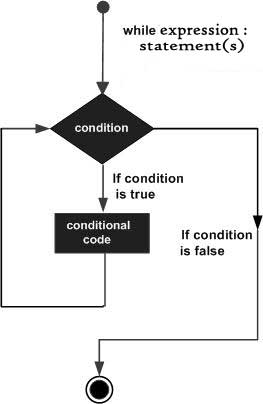
\includegraphics[width=0.3\textwidth]{fig_python_1}
		\caption{The control flow of a while loop}
		\label{fig_python_1}
	\end{center}
\end{figure}

Below we provide a simple example.

\begin{lstlisting}[language=Python]
#Example 
>>> x = 10       # assign an initial value to x
    print(x)     # prints the initial value
    while x > 1: # as long as x is bigger than 1:
   	x=x/2    #      - divide x by 2
   	print(x) #      - print the new value of x
   	
 10
 5.0
 2.5
 1.25
 0.625
\end{lstlisting}

Note that if the condition is always met, the program will be stuck in a while loop and must be aborted manually. This can be done via \textbf{Kernel > Interrupt}.

\subsubsection{For-loop}

A second control statement is the \textbf{for-loop}. This repeats, like the while loop, a number of operations. However, the number of iterations here is predefined by the so-called \textbf{iterator}. This iterator iterates through the elements of a specified set of data. In Python, we write a for loop as:

\begin{lstlisting}[language=Python]
	for element in iterator:
	    operations 
\end{lstlisting}

The expressions within the for-loop are also grouped together. The control flow is illustrated in Figure~\ref{fig_python_2}.

\begin{figure}[H]
	\begin{center}
		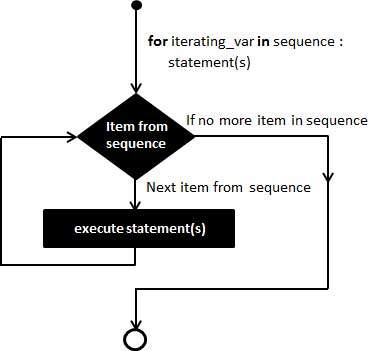
\includegraphics[width=0.3\textwidth]{fig_python_2}
		\caption{Controlflow of a for-loop.}
		\label{fig_python_2}
	\end{center}
\end{figure}

\begin{lstlisting}[language=Python]
#example
>>> for value in [1,2,3,4]:
        print(value)

 1
 2
 3
 4
\end{lstlisting}

A for-loop can be used to quickly create lists.
\begin{lstlisting}[language=Python]
	new_list = [operation with element for element in iterator] 
\end{lstlisting}


\begin{lstlisting}[language=Python]
#example 
>>> l_1 = [1,2,3,4]
    l_2 = [value**2 for value in l_1] #squares the values in list l_1
    l_2

[1, 4, 9, 16]
\end{lstlisting}

\subsubsection{If, else-control statement}

Finally, we discuss the decision structure \textbf{if}. This imposes a certain condition that must be met before a sequence of operations may be performed. In Python, we enter this as follows.

\begin{lstlisting}[language=Python]
	if condition == True:
	    operations    
\end{lstlisting}

The control flow is illustrated in Figure~\ref{fig_python_3}.

\begin{figure}[H]
	\begin{center}
		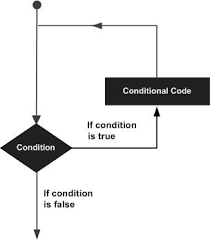
\includegraphics[width=0.3\textwidth]{fig_python_3}
		\caption{Control flow of an if-statement.}
		\label{fig_python_3}
	\end{center}
\end{figure}

In order to perform different operations depending on whether a condition is met or not, we can also use \textbf{else}. Then, we specify the operations to be performed if the condition is not met.

\begin{lstlisting}[language=Python]
	if condition == True:
	    operations # are executed if condition was met
	else:
	    operations # are executed if condition was not met    
\end{lstlisting}

The expressions within if and else are aligned in the same way. 

\begin{lstlisting}[language=Python]
#Example 
>>> cd = True
    if cd:
        print("The condition was met")
    else:
        print("The condition was not met")
        
    The condition was met
\end{lstlisting}

\section{Packages}
In addition to the basic syntax, Python has numerous additional functionalities. These are collected in so-called \textbf{packages}, which can be loaded via:

\begin{lstlisting}[language=Python]
	import package as packagename
\end{lstlisting}

This makes that all the definitions in the package are stored in the variable \lstinline|packagename|. Next, when we want to use a function from the imported package, we do so as follows:

\begin{lstlisting}[language=Python]
	packagename.functionname()
\end{lstlisting}

We can also import the function straight from the package using \lstinline|from|:

\begin{lstlisting}[language=Python]
	from package import functiename
\end{lstlisting}

after which we can call the function directly:

\begin{lstlisting}[language=Python]
	functiename()
\end{lstlisting}

The input cell below loads a number of packets.

\begin{lstlisting}[language=Python]
import numpy as np 
import matplotlib.pyplot as plt
from ipywidgets import interact, fixed
\end{lstlisting}

\subsection{Numpy}
Numpy is the package that provides the foundation for scientific programming in Python. It contains numerous mathematical functions and numbers, such as:
\begin{itemize}
	\item trigonometric functions: \lstinline|np.sin(), np.cos()| \ldots
	\item exponential and logarithmic functions: \lstinline|np.exp(), np.log()|
	\item the number $\pi$ : \lstinline|np.pi|
\end{itemize}

\subsection{Sympy}

\subsection{Other Packages}
In addition to Numpy, a number of other packages can be loaded:

\begin{itemize}
	\item \lstinline|matplotlib.pyplot| to make figures
	\item \lstinline|ipywidgets| to make these figures interactive
\end{itemize}
